\documentclass[12pt,a4paper]{article}
\usepackage{times}
\usepackage{durhampaper}
\usepackage{harvard}
\usepackage{graphicx}
\usepackage{longtable}

\citationmode{abbr}
\bibliographystyle{agsm}

\title{Enigma and BOMBE simulation}
\author{A.L. Gillies}
\student{A.L. Gillies}
\supervisor{M. Johnson}
\degree{MEng Computer Science}

\date{}
\begin{document}
\maketitle

\begin{abstract}\\

{\bf Context/Background} - Can antiquated ideas and designs be brought to the modern day? The aim of this paper is to show the plausibility of this using the Enigma and the BOMBE, two cryptographic devices from the second world war, these will be modernised and tested to prove this hypothesis.\\

{\bf Aims} - Using the known execution speed of the antique Engima and BOMBE, the aim of this paper is to show, through implementation and testing of a modern interpretation of the Enigma and BOMBE, the speed up that has occurred since the inception of both.\\

{\bf Method} - After both the Engima and BOMBE are implemented the BOMBE will then be improved on using parallelisation techniques. Each will then be tested. The time taken for a standard engima machine to encrypt, the computerised version to encrypt and the parallelised version to encrypt will be compared to one another to give a good indication of the improvements over time. Another comparison will be made between the standard Enigma, the computerised Enigma and the parallelised Enigma, this should re-enforce the indication of computer improvements.\\

{\bf Proposed Solution} - The Enigma machine will be implemented through C++ code, this will form the baseline for a modern interpretation of the machine as it will not run anything in parallel. This code will then be parallelised using different standardised techniques, these will then be used as the final comparison to show the significant increases in performance that this seemingly antiquated idea can expect across different inputs.\\
\end{abstract}

\begin{keywords}
Enigma, BOMBE, Parallel, Modern, Computation, Evaluation, Reinterpretation, Comparison, C++, Antiquated.
\end{keywords}



\section{Introduction}

\subsection{Description and Purpose}

This project is to be an investigation into the possible improvements that can be gained on an antiquated technique by parallelisation against unparallelised and a time accurate representation. This will be done by first creating a modern equivalent of the antiquated technique. The modern equivalent will then be improved upon using parallelisation techniques. This is to be done on the BOMBE using the Enigma machine.

\subsection{What is the Enigma Machine?}

The Enigma machine was an early to mid 20th century cryptography device, it was used in both commercial and military applications. Most famous for its use by Nazi Germany during the second world war, the electro-mechanical rotor device was made up of three rotors, a plugboard, and a reflector. The user interface for the device is a keyboard and a lightboard, once a letter is pressed on the keyboard, it is then encrypted and the corresponding encrypted letter will light up on the lightboard. 

The device encrypts any given letter is the same way. Once a letter has been pressed on the keyboard a signal is passed through the plugboard this is a plug-based one to one mapping of all the letters on the keyboard to a unique letter of the alphabet. This output is then passed to the first of three rotors, a rotor is a set one to one mapping that will then step to the next letter once used. The order of either alphabet on the rotor cannot be changed but the mapping of the input letter to the output letter will change after each time it is used, this is called the stepping mechanism. The first rotor will step each time a letter is pressed and the second will only step if the first rotor has done a complete rotation, the third will only step if the second has done a complete rotation. The final component is the reflector this is similar to the plugboard that it is a one to one mapping but has the issue that it cannot map a letter to itself. After the reflector the signal is sent back through all three rotors and then through the plugboard to light up one of the letters on the lightboard. 

The device has several settings that can be changed. Firstly the plugboard is reprogrammable, the plugboard is a one to one mapping between two alphabets. Secondly, the device typically has three rotors that can be used at any one time, there are eight rotors that can be put in any one of the three position, left, right and centre. Having chosen three of the rotors and their positions in the device, the initial rotation of each also has to be chosen. Finally, the reflector is also programmable, this is another one to one mapping between two alphabets.

\begin{figure}[h]
\centering
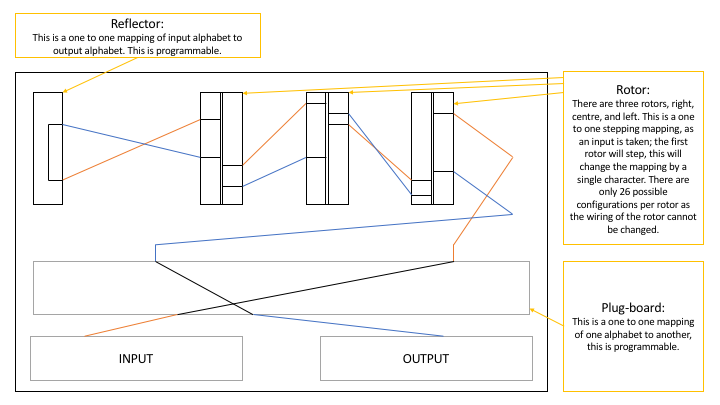
\includegraphics[width=\textwidth]{enigmaDiagram.png}
\end{figure}

\subsection{What is the BOMBE?}

The BOMBE is the antithesis of the Engima machine, it was specifically designed by British cryptologists in 1939 to counter the Enigma encoded messages that were used by the Axis at the time. The BOMBE was designed to to discover the settings used by the Enigma operators that were changed daily. 

The BOMBE was an electro-mechanical device that replicated the action of several Enigma machines wired together; the British BOMBE contained 36 Enigma representations.

The BOMBE was based on the probably-phrase attack; it is possible to exploit the relationship between a section of plaintext that was either guessed or already known, and the ciphertext to which it might correspond. The idea of the BOMBE was to remove any superfluous Enigma set-ups using the fact that the Enigma could not encode a letter as itself. Once the 'crib' or the guessed plaintext had been shown to be the test ciphertext then the settings of the Enigma would be known and any other messages sent by the Enigma machines would be known for the rest of the day as the British cryptologists knew the settings used for the current messages and it was just a case of feeding the ciphertext into their own Enigma machine with the current settings and reading the output.

The crib is shown to correspond to the ciphertext through several steps. The first is to use the fact that the Enigma had a flaw in the encryption process to full effect, if at any point the same letter is in the same position in the ciphertext and crib then this encryption is invalid thus the crib will be moved one letter over and retested, this removed a lot of unnecessary testing in the later stages. 

To give a visual representation of the first stage.

\begin{figure}[h]
\centering
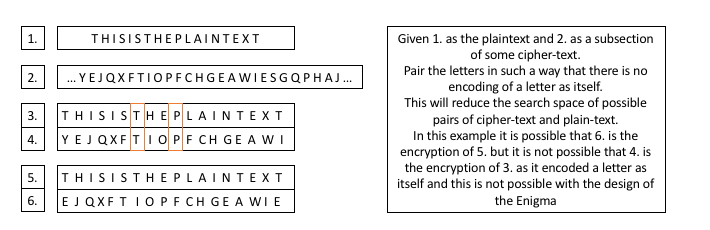
\includegraphics[width=\textwidth]{StageOneBOMBE.png}
\end{figure}

The second stage is to create a connection network for each step, this is done by pairing and numbering a possible ciphertext-plaintext pair and creating a network where any pairing is a transition pair in the ciphertext-plaintext pair.

An example of what the connection network could look like is shown bellow.

\begin{figure}[h]
\centering
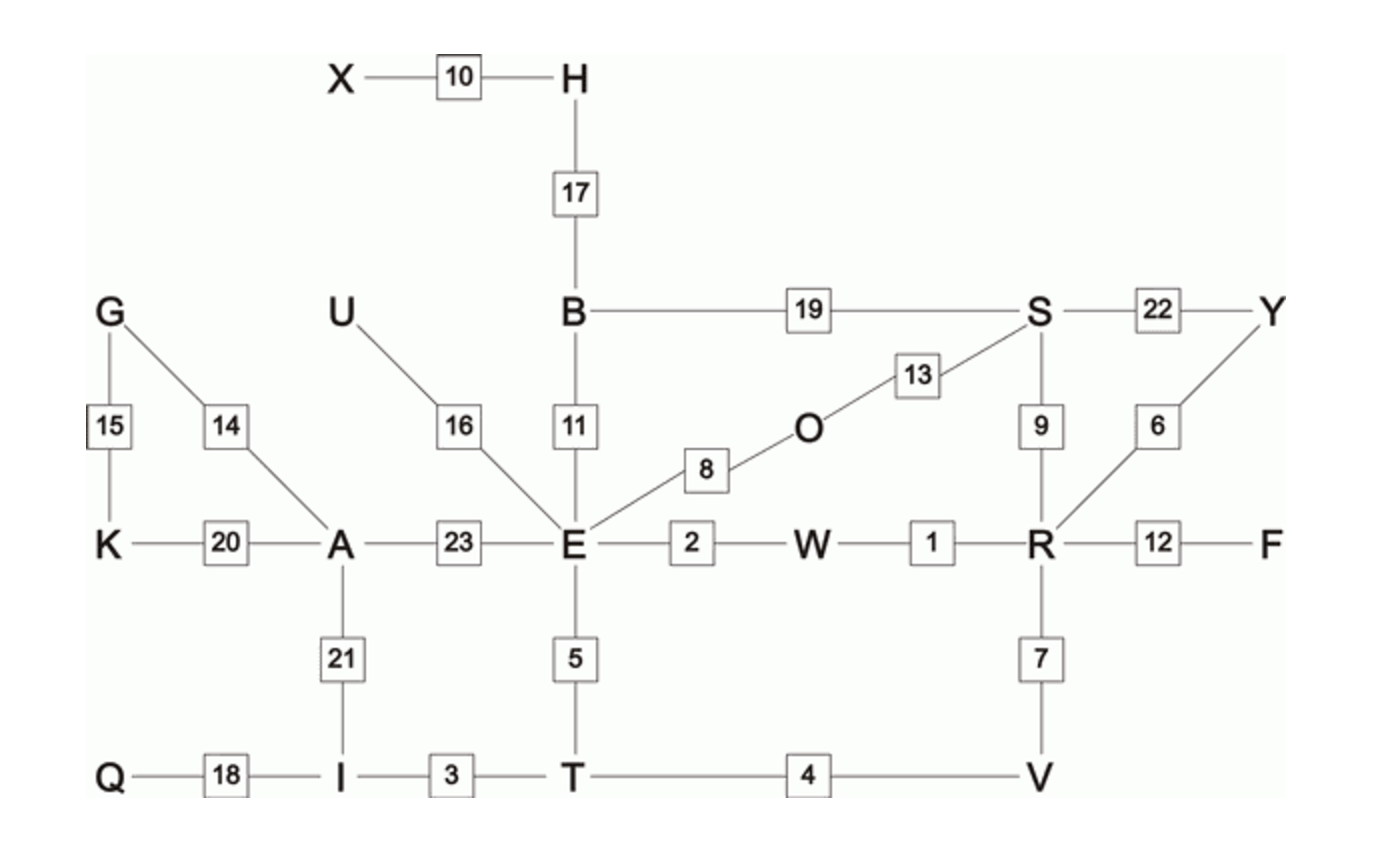
\includegraphics[width=\textwidth]{StageTwoBOMBE.png}
\end{figure}

...
talk about the other stages of the BOMBE and detail this one
...

\subsection{What are the parallelisation techniques?}

With the way the BOMBE works, over a set alphabet in a sequential nature, parallelisation would be a marked improvement as it would allow for a search over the set alphabet in a non-sequential way and thus improve speed. There are several techniques that could be employed to improve the speed of the search. Single Instruction Multiple Data is a idea that is rooted in doing the same instruction to multiple data sources, for example, if one wanted to add six to a lot of numbers, an unparallelised program would load the first number then add to it and send it back, a parallelised program would load as many of the numbers as it could, add six to all of them in one go then send them back. Multiple Instruction Multiple Data is another parallelisation technique that is much harder to implement but has the added benefit that different operations can be done to different datasets so two almost unconnected tasks can be done simultaneously. 

...
keep writing
...

\subsection{Deliverables}

\subsubsection{Minimum Objectives}

- Simulate Enigma and show its correctness, by encrypting plaintext and comparing this to its known ciphertext to show this correctness, this should be done over a significant database of plaintext and ciphertext.\\
- Simulate BOMBE and show its correctness, taking some of the aformentioned stock ciphertext and running the BOMBE on this input such that the plaintext is output as the result.

\subsubsection{Intermediate Objectives}

- Prove the correctness of the Enigma simulation by encrypting plaintext and comparing this to its known ciphertext to show this correctness. This should be done over a significant database of plaintext and corresponding  ciphertext.\\
- Prove that the BOMBE simulation is correct by taking all of the aformentioned stock ciphertext and running the BOMBE on this input such that the plaintext is output as the result.\\
- Both simulations should also be proved to be effective on random inputs and also in relation to one another; the Enigma machine should be run on a random input and the output should then be used as the input on the BOMBE which should in turn return the random plaintext.\\
- Evaluate average computational time on inputs of a set size.

\subsubsection{Advanced Objectives}

- Increase the scope of the BOMBE simuation by running the simulation in parallel. This means that different parts of the ciphertext could be run in parallel or the whole cipher text being run with each parallel part testing different configurations of the Engima machine.



\section{Design}

\subsection{Tools}

The only tools I will need are the Intel compiler, this will allow for the unimproved version of both the Enigma and BOMBE to be written in C++ meaning that it can be compiled by a standard C++ compiler. The Intel tools will allow for parallelisation techniques to be applied to the BOMBE simulation, at this point only the intel compiler will be able to compile the code to fully utilise the additions to the code that parallelization require. I have chosen C++ as my base language mainly because it has an expansive library of parlallel tools, this is the intel comiler, and it is also a language I am very familiar with, having used it extensively throughout my academic career.

\subsection{Development and Maintenance}

The project will be designed and produced in an agile manner, it will also incorporate a modular progression. Each system, Enigma and BOMBE, will be produced independent of one another. This will allow verification of correctness to be acquired at several different stages throughout the implementation and not as a final progression. The Engima machine will be designed and implemented first, it will then be verified. Following that the standard BOMBE will be implemented and using the already verified engima as a means to show to correctness of the BOMBE, it will also be tested on known (ciphertext, plaintext) pairs as well. This will lead onto the final stage, the parallelisation and testing of the BOMBE, it will continuously be verified during this process to produce a fast and correct BOMBE implementation that will then be tested against it unparallelised counterpart, leading to a conclusion.

The maintenance of this system will most likely not extend far past the deadline date, as by this point both systems will be fully working in the latest version of the intel compilers and will not be changed for any updated version of the compilers. The systems will work on any operating system that can install the latest version of the intel compilers at the time of the deadline.

\subsection{System Architecture and Design}

The system will consist of two stand alone C++ programs, each will have an input file that will tune parameters and inputs. Each system will have a shell script that will verify the inputs, recompile on the current system, tune the parameters and then run the system with these settings. This will be the same for both the Enigma and BOMBE. The settings file will be in the form of a basic .txt file, this will have a standard format. The settings file will contain; which rotors to use in which positions, what their offset is, the plugboard and reflector mappings, as well as the plaintext. 

Neither the Enigma or the BOMBE will allow for continuous input of characters as the plaintext or ciphertext respectively as this would be the dictate of the speed of the system, the characters cannot be input fast enough for there to be no machine idle time between two adjacent characters. Thus rendering a timed run completely dependant on how fast the user can type and not on the system itself.

The Enigma simulation will output its results to a text file as this will be useful for comparison as well as using the output of the Enigma simulation as the input for the BOMBE simulation as well as having files for both the cipher-text and plain-text that will form the basis of the testing of both simulations. The BOMBE will also output a text file as a result as, again, this will be useful for testing at a later date. 

\subsection{Functional Requirements}

\begin{table}[htb]
\centering
\caption{Functional Requirements}
\vspace*{6pt}
\label{units}
\begin{longtable}{ |p{3cm}|p{3cm}|p{3cm}|p{3cm}| }\hline\hline
Unique ID & Deliverable & Description & Priority \\ \hline
DL1 & Simulate the Enigma Machine & Have a working Enigma machine that can take in settings and plaintext and return ciphertext. & High \\ \hline
DL2 & Simulate the Bombe & A working BOMBE that takes in settings and ciphertext and returns decoded plaintext. & High \\ \hline
DL3 & Show the correctness of the Enigma Machine & Show through a series of tests and validations that the plaintext fed to the Enigma Machine and the Ciphertext returned are paired through the settings of the enigma & Medium \\ \hline
DL4 & Show the correctness of the BOMBE & Show that the known plaintext of the ciphertext input into the BOMBE is exactly the same as the plaintext that is returned by the BOMBE & Medium \\ \hline
DL5 & Evaluate average computation time over set inputs for both Enigma and BOMBE & Using a wide range of known plaintext - ciphertext pairs find the average computation time, the time take on average to do a single encode or decode for both simulations & High \\ \hline
DL6 & Parallelise The BOMBE and evaluate average computation time & Using known parallelisation techniques increase the speed at which the BOMBE will decode a given ciphertext & High \\ \hline
\end{longtable}
\end{table}

\subsection{Evaluation}

Each system will be evaluated individually first then in conjunction to one another. To evaluate the Enigma, it will be tested over known (plaintext,ciphertext) pairs to show output is valid. The BOMBE is tested over known and unknown ciphertext, the output of the known ciphertext will then be reencrypted using the settings that were used to decrypt it and they will be compared to show correctness. Once correctness has been established then decryption time will compared between the parallelised and standard BOMBE over the same ciphertext.

\subsection{References}

\bibliography{projectpaper}

...
format document
...

\end{document}